% Mostrar el grado de cumplimiento de los objetivos
\section{Resultados}
Se logró implementar la totalidad del juego especificado en la Sección~\ref{sec:diseño}. El link al ejecutable se puede encontrar en \url{https://drive.google.com/file/d/1bRaYZMCMvfS-mlVrCAlm8tI2Kh1XUgZM}.

\begin{figure}[h]
    \centering
    \begin{minipage}{.24\textwidth}
        
\includegraphics[width=\textwidth]{imgs/pantalla-inicio.png}
    \end{minipage}
    \begin{minipage}{.24\textwidth}
        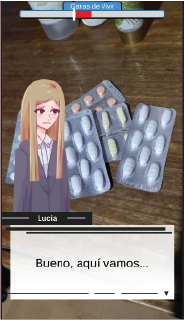
\includegraphics[width=\textwidth]{imgs/screenshot-final1.png}
    \end{minipage}
    \begin{minipage}{.24\textwidth}
        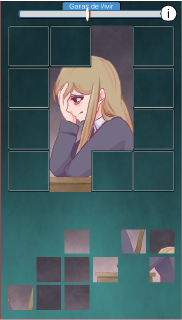
\includegraphics[width=\textwidth]{imgs/screenshot-final2.png}
    \end{minipage}
    \begin{minipage}{.24\textwidth}
        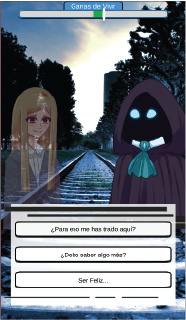
\includegraphics[width=\textwidth]{imgs/screenshot-final3.png}
    \end{minipage}
    \caption{Screenshots del juego terminado}
    \label{fig:screenshots-terminado}
\end{figure}

El resto de las pantallas implementadas se pueden ver en la Sección~\ref{sec:pantallas} de Diseño.

%\textbf{ESTE APARTADO SE REFIERA AL RESULTADO DEL JUEGO COMO PRODCUTO FINAL. PON UN LINK CON UNA DEMO O UN LINK  AUN EJECUTABLE. SI QUIERES PON ALGUNA CAPTURA DE PANTALLA O INDICA QUE LAS PANTALLAS DEL JUEGO SE PUEDEN VER EN LA SECCIÓN DE DISEÑO}


%\textbf{para mi este apartado son comentarios de los usarios finales. Si quieres pones como titulo la opicion de los jugadores sobre el juego.} 

\subsection{Opiniones de los Usuarios}
El juego recibió críticas mayormente positivas de parte de los usuarios que lo probaron. En las Figuras~\ref{fig:testimonio1}, \ref{fig:testimonio2} y~\ref{fig:testimonio3} se adjuntan algunos testimonios de los jugadores.

\begin{figure}[ht]
    \centering
    
\includegraphics{imgs/feedback.png}
    \caption{Testimonio 1}
    \label{fig:testimonio1}
\end{figure}

\begin{figure}[ht]
    \centering
    
\includegraphics{imgs/feedback2.png}
    
\includegraphics{imgs/feedback3.png}
    \caption{Testimonio 2}
    \label{fig:testimonio2}
\end{figure}

\begin{figure}[ht]
    \centering
    
\includegraphics{imgs/feedback7.png}
    \caption{Testimonio 3}
    \label{fig:testimonio3}
\end{figure}

% TO DO: ANALIZAR Y AÑADIR GRAFICOS DE LOS DATOS
\subsection{Investigación}
Por el lado de la investigación, se recopilaron datos de 48 usuarios distintos. De estos usuarios la mayoría es Hombre (70.8\%), de entre los 18 y 22 años de edad (56.3\%) y proveniente de Chile (89.6\%), como se puede ver en la Figura~\ref{fig:demografia}.


%\textbf{TIENES LOS RESULTADOS PREGUNTA POR PREGUNTA? CREO QUE TAMBIEN SERIA INTERESANTE I LO QUE PRESENTAS A CONTINUACIÓN ES MAS COMO UNA VALORACIÓN GLOBAL. LO DIGO PORQUE SI TIENES LOS DATOS VALE LA PENA PONERLOS.}

\begin{figure}[h]
    \centering
    \begin{minipage}{.5\textwidth}
        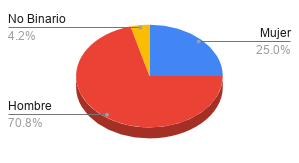
\includegraphics[width=\textwidth]{imgs/chart-genero.png}
    \end{minipage}
    \begin{minipage}{.42\textwidth}
        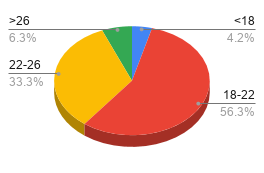
\includegraphics[width=\textwidth]{imgs/chart-edad.png}
    \end{minipage}
    \begin{minipage}{.55\textwidth}
        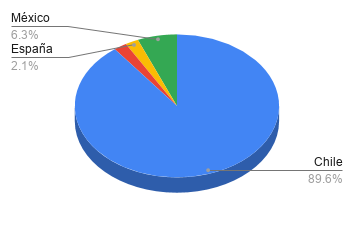
\includegraphics[width=\textwidth]{imgs/chart-pais.png}
    \end{minipage}
    \caption{Datos Demográficos}
    \label{fig:demografia}
\end{figure}

\subsubsection{Decisiones in-game}

Lo primero que se puede ver en la Figura~\ref{fig:decision} es que la mayoría de los jugadores mantuvo la decisión original que habían tomado (70.8\% vs 29.2\%), sin embargo, este dato se vuelve más interesante cuando vemos un poco más allá y separamos los datos según la decisión inicial de los usuarios.

\begin{figure}[h]
    \centering
    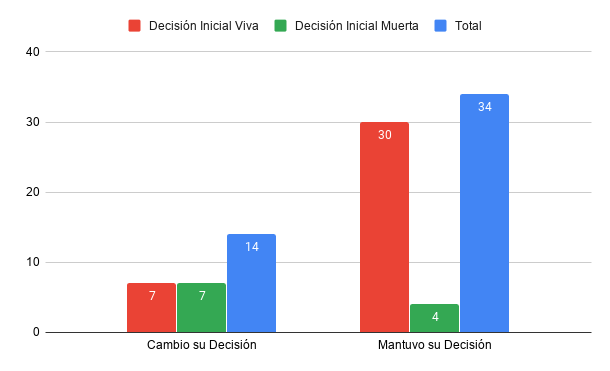
\includegraphics[scale=0.7]{imgs/resultado-decision.png}
    \caption{Cantidad de Jugadores que cambiaron o mantuvieron su decisión inicial.}
    \label{fig:decision}
\end{figure}

En el caso de los jugadores que salvaron a Lucía inicialmente, la mayoría (81\%) optó por mantenerla viva al final del juego.

Pero cuando miramos a los jugadores que eligieron que Lucía muriera inicialmente, la mayoría (63.6\%) cambió de decisión y eligió que viviera al final del juego.

\subsubsection{Resultados Cuestionario}

Para esta investigación se utilizó el \acrlong{mfq}\cite{moral-foundation}, un cuestionario que permite entender la moralidad desde 5 pilares fundamentales. En este caso en particular veremos la variación de puntaje en el pilar de Afecto/Daño, el cuál está relacionado a los sistemas de empatía y apego que sienten las personas por otras. Este puntaje es la suma de las respuesta de los usuarios en 6 preguntas en particular.

Las preguntas relacionadas a este pilar son las siguientes:
\begin{itemize}
    \item Cuando decides si algo está bien o mal, ¿Qué tan relevantes son las siguientes consideraciones para tu juicio?
    \begin{itemize}
        \item 1. Si alguien sufre (o no) emocionalmente.
        \item 7. Si alguien se preocupa (o no) por el débil y vulnerable.
        \item 12. Si alguien es (o no) cruel.
    \end{itemize}
    \item Señala tu acuerdo (5) o desacuerdo (0) con las siguientes oraciones:
    \begin{itemize}
        \item 17. La compasión por los que sufren es la virtud más importante.
        \item 23. Una de las peores cosas que una persona puede hacer es dañar a un animal indefenso.
        \item 28. Nunca será correcto matar a un ser humano
    \end{itemize}
\end{itemize}

A continuación veremos los datos en detalle pregunta por pregunta.

\paragraph{Pregunta 1. Si alguien sufre (o no) emocionalmente}
La Figura~\ref{fig:chart-p1} nos muestra como variaron las respuestas en ambas encuestas, podemos ver que los usuarios tendieron a mantener o aumentar su respuesta, lo que indica una influencia por parte del juego.

\begin{figure}[h]
    \centering
    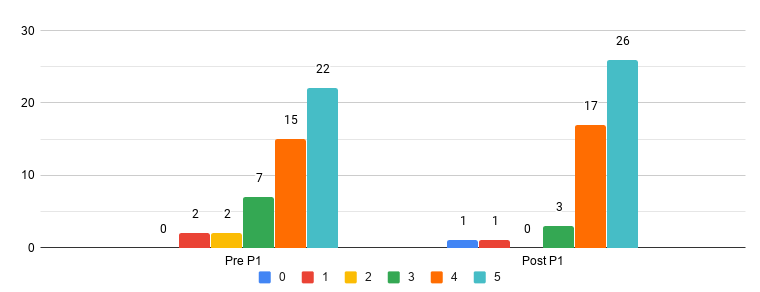
\includegraphics[width=.9\textwidth]{imgs/chart-p1.png}
    \caption{Respuestas Pregunta 1}
    \label{fig:chart-p1}
\end{figure}

\paragraph{Pregunta 7. Si alguien se preocupa (o no) por el débil y vulnerable}
La Figura~\ref{fig:chart-p7} nos muestra un comportamiento similar al de la pregunta anterior, donde las respuestas subieron de [4]~Muy Relevante a [5]~Extremadamente Relevante.

\begin{figure}[h]
    \centering
    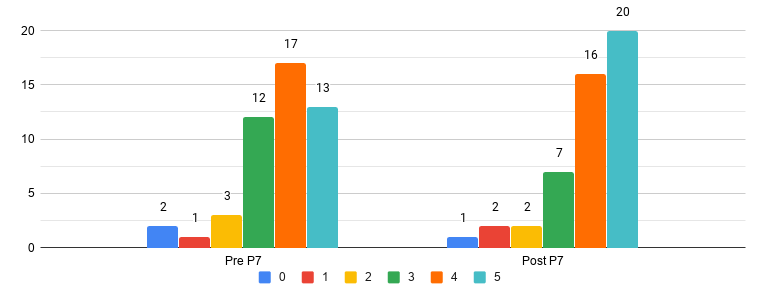
\includegraphics[width=.9\textwidth]{imgs/chart-p7.png}
    \caption{Respuestas Pregunta 7}
    \label{fig:chart-p7}
\end{figure}

\paragraph{Pregunta 12. Si alguien es (o no) cruel}
La Figura~\ref{fig:chart-p12} unos cambios divididos, vemos que hubieron cambios hacia [5]~Extremadamente Relevante, pero también vemos a algunos usuarios irse hacia [1]~No muy Relevante.

\begin{figure}[h]
    \centering
    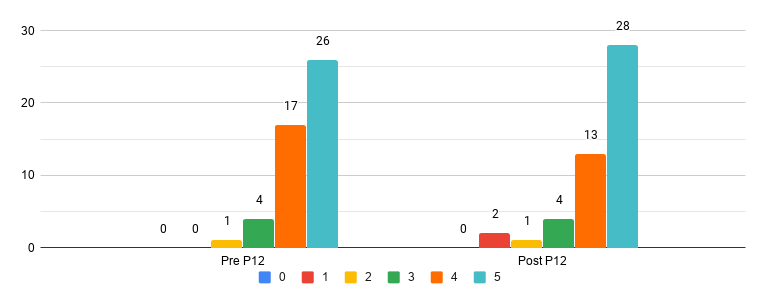
\includegraphics[width=.9\textwidth]{imgs/chart-p12.png}
    \caption{Respuestas Pregunta 12}
    \label{fig:chart-p12}
\end{figure}

\paragraph{Pregunta 17. La compasión por los que sufren es la virtud más importante}
La Figura~\ref{fig:chart-p17} nos muestra un incremento general en la opinión de los jugadores, podemos ver que se movieron de [2]~Levemente en desacuerdo y [3]~Levemente de acuerdo hacia [4]~Moderadamente de acuerdo y [5]~Muy de acuerdo

\begin{figure}[h]
    \centering
    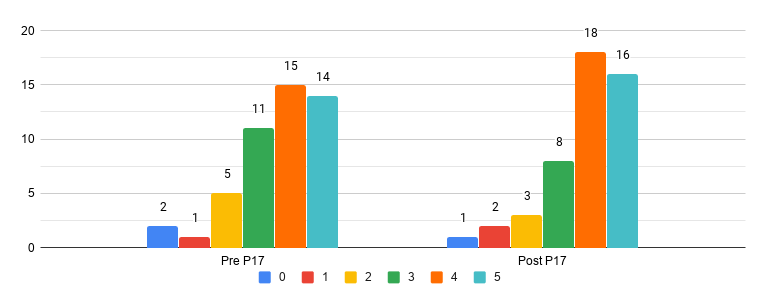
\includegraphics[width=.9\textwidth]{imgs/chart-p17.png}
    \caption{Respuestas Pregunta 17}
    \label{fig:chart-p17}
\end{figure}

\paragraph{Pregunta 23. Una de las peores cosas que una persona puede hacer es dañar a un animal indefenso}
La Figura~\ref{fig:chart-p23} nos muestra 2 cambios relevantes: el primero es el aumento de [5]~Muy de acuerdo, y el segundo es el aumento de [1]~Moderadamente en desacuerdo y [3]~Levemente de acuerdo. Esto podría indicar una inclinación más neutra de parte de algunos usuarios después de haber experimentado el juego.

\begin{figure}[h]
    \centering
    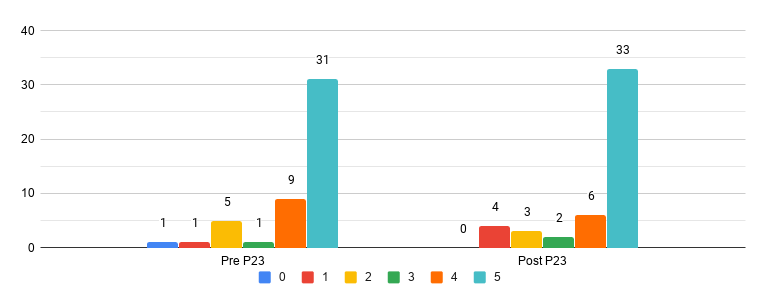
\includegraphics[width=.9\textwidth]{imgs/chart-p23.png}
    \caption{Respuestas Pregunta 23}
    \label{fig:chart-p23}
\end{figure}

\paragraph{Pregunta 28. Nunca será correcto matar a un ser humano}
La Figura~\ref{fig:chart-p28} nos muestra la primera baja de [5]~Muy de acuerdo a lo largo de las 6 preguntas, junto con un aumento de [3]~Levemente de acuerdo y [4]~Moderadamente de acuerdo. Esto nos puede indicar que los jugadores se cuestionaron la muerte, y el suicidio como una opción potencialmente válida después de haber jugado el juego.

Recordemos que la mayoría eligió mantener a Lucía viva al inicio, por lo que se enfrentaron a la ruta del juego que les trataba de influenciar para creer en el suicidio como algo válido.

\begin{figure}[h]
    \centering
    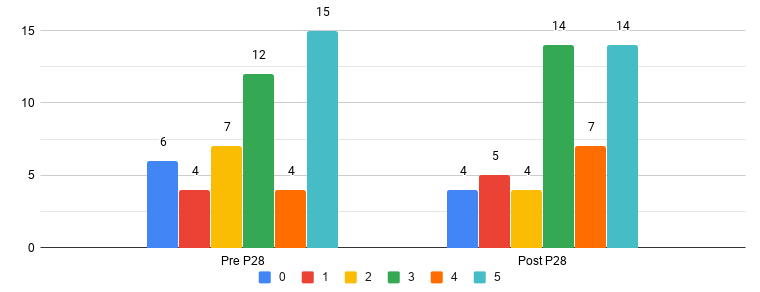
\includegraphics[width=.9\textwidth]{imgs/chart-p28.png}
    \caption{Respuestas Pregunta 28}
    \label{fig:chart-p28}
\end{figure}

\paragraph{Resultados Generales}
En general los jugadores mostraron un aumento en sus respuestas después de haber jugado al juego, lo que nos puede indicar que el juego influyó en su moral y les hizo -al menos- cuestionarse la muerte y la empatía que tienen hacia otras personas.

La Figura~\ref{fig:encuesta-resultados} nos muestra como fue la variación de los resultados de las encuesta según la decisión original de los jugadores. Es interesante apreciar como estos resultados aumentaron o disminuyeron casi en su totalidad (91.7\%), lo que nos muestra que los jugadores no fueron indiferentes al videojuego y su narrativa.

\begin{figure}[h]
    \centering
    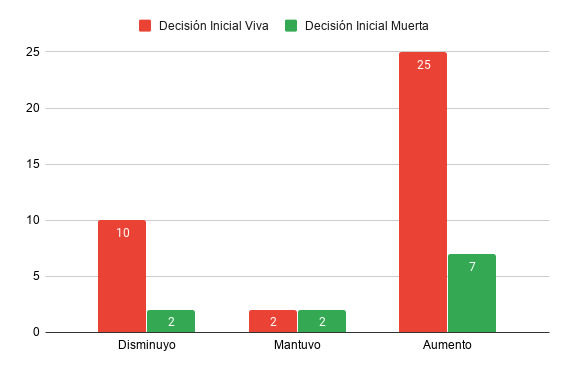
\includegraphics[scale=.7]{imgs/resultado-encuesta-separado.png}
    \caption{Variación en el resultado de las encuestas}
    \label{fig:encuesta-resultados}
\end{figure}

%Al ver los datos de la Figura~\ref{fig:encuesta-general}, un 91\% de las personas tuvo una variación en su puntaje lo que nos indica que el juego les influyó de una manera u otra, particularmente a ese 66\% de las personas que tuvieron un aumento en la puntuación de su encuesta.

%\begin{figure}[h]
%    \centering
%    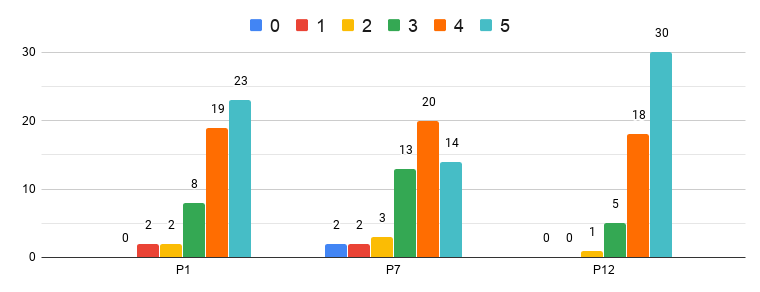
\includegraphics[width=\textwidth]{imgs/chart.png}
%    \caption{Cantidad de Jugadores que cambiaron o mantuvieron su decisión inicial.}
%\end{figure}

%\begin{figure}
%    \centering
%    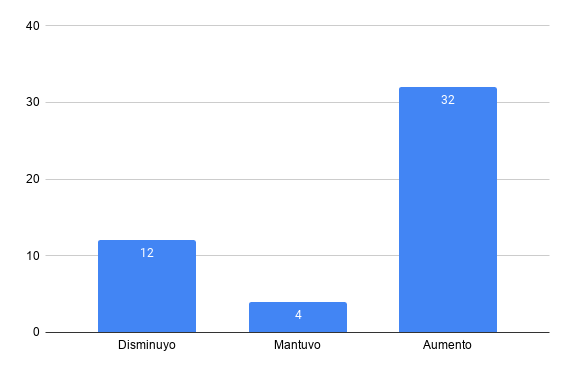
\includegraphics[scale=0.7]{imgs/resultado-encuesta-general.png}
%    \caption{Variación en el puntaje de las encuestas}
%    \label{fig:encuesta-general}
%\end{figure}

%Si vemos los resultados de estas encuestas separados por la decisión inicial que tomaron los jugadores tal como aparece en la Figura~\ref{fig:encuesta-separado}, vemos una tendencia similar en ambas rutas, las cuales nos muestran que un 68\% y un 63\% de los jugadores que jugaron su respectiva ruta mostraron un incremento en su \textbf{puntaj\textbf{e.}(TE REFIERES A PUNTUACIÓN????)}

%\begin{figure}
%    \centering
%    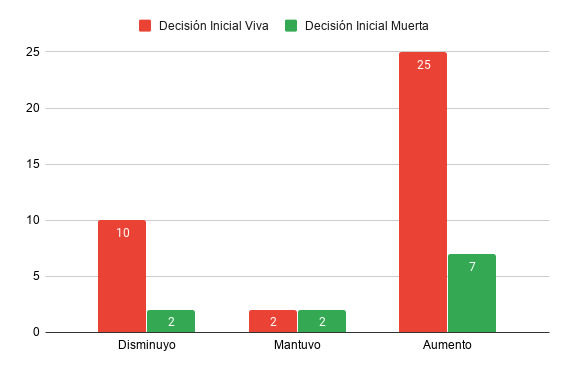
\includegraphics[scale=0.7]{imgs/resultado-encuesta-separado.png}
%    \caption{Variación en el puntaje de las encuestas según decisión inicial}
%    \label{fig:encuesta-separado}
%\end{figure}